\begin{table*}
\begin{tabular*}{\textwidth}{>{\bfseries}l >{\bfseries}l @{\extracolsep{\fill}}>{\hspace{2em}}r r r r r r >{\hspace{2em}}r >{\hspace{-1em}}r}
\multicolumn{10}{>{\bfseries}c}{Full Graph} \\
\toprule
Model & Level & Accuracy & Precision & Recall & AUC & F\textsubscript{1}-score & F\textsubscript{4}-score & Fit Time & Predict Time \\
\midrule

\multicolumn{2}{>{\bfseries}l}{Random Selection}
& 0.499 & 0.499 & 0.500 & 0.499 & 0.500 & 0.500 & \NA{} & \SI{0.005}{\second} \\

\multicolumn{2}{>{\bfseries}l}{Majority Voting}
& 0.565 & 0.747 & 0.197 & 0.565 & 0.312 & 0.206 & \NA{} & \SI{0.204}{\second} \\
\midrule

\multirow{5}{*}{LR}
& $\ego_1$ & 0.534 & 0.586 & 0.234 & 0.534 & 0.335 & 0.243 & \SI{0.937}{\second}   & \SI{0.016}{\second} \\
& $\ego_2$ & 0.547 & 0.617 & 0.250 & 0.547 & 0.356 & 0.260 & \SI{1.347}{\second}   & \SI{0.035}{\second} \\
& $\ego_3$ & 0.563 & 0.586 & 0.430 & 0.563 & 0.496 & 0.437 & \SI{1.055}{\second}   & \SI{0.023}{\second} \\
& $\cat_1$ & 0.565 & 0.746 & 0.198 & 0.565 & 0.313 & 0.207 & \SI{1.871}{\second}   & \SI{0.041}{\second} \\
& $\cat_2$ & 0.577 & 0.727 & 0.247 & 0.577 & 0.368 & 0.257 & \SI{9.816}{\second}   & \SI{0.077}{\second} \\
& $\cat_3$ & 0.589 & 0.636 & 0.415 & 0.589 & 0.503 & 0.424 & \SI{9.456}{\second}   & \SI{0.065}{\second} \\
\midrule

\multirow{5}{*}{RF}
& $\ego_1$ & 0.543 & 0.544 & 0.529 & 0.543 & 0.536 & 0.530 & \SI{25.789}{\second}  & \SI{4.878}{\second} \\
& $\ego_2$ & 0.578 & 0.585 & 0.537 & 0.578 & 0.560 & 0.540 & \SI{102.961}{\second} & \SI{5.608}{\second} \\
& $\ego_3$ & 0.583 & 0.590 & 0.541 & 0.583 & 0.564 & 0.543 & \SI{70.447}{\second}  & \SI{3.148}{\second} \\
& $\cat_1$ & 0.568 & 0.573 & 0.536 & 0.568 & 0.554 & 0.538 & \SI{32.981}{\second}  & \SI{5.371}{\second} \\
& $\cat_2$ & 0.613 & 0.634 & 0.533 & 0.613 & 0.579 & 0.538 & \SI{44.911}{\second}  & \SI{6.002}{\second} \\
& $\cat_3$ & \textbf{0.614} & 0.635 & 0.534 & \textbf{0.614} & \textbf{0.580} & \textbf{0.539} & \SI{50.589}{\second}  & \SI{3.484}{\second} \\
\bottomrule
\end{tabular*}
\caption{Resulting metrics of different methods used in \cref{sec:results} tested on both the \emph{Full Graph}, which includes all the nodes of the graph. \textbf{LR} corresponds to \emph{Logistic Regression} models, and \textbf{RF} to \emph{Random Forest} ones with the level described in \cref{sec:accumulatedfeatures}. \textbf{Bolded} items represent the highest value for each metric which is being presented in this paper.}
\label{tab:fullgraphresults}
\end{table*}


\section{Inference Methodology}
\label{sec:inference_methodology}

As previously explained in \cref{subsec:categoricaluserdata}, the nodes in $T \subseteq V$ are separated into two disjoint subgroups, $G$ and $H$, so that $G \cup H = T$, $G \cap H = \varnothing$, $\left| G \right| = 0.75 \cdot \left| T \right|$, and $\left| H \right| = 0.25 \cdot \left| T \right|$. Furthermore, the subset $H_{\inner} \subseteq H$ is defined so that a node $h \in H_{\inner}$ if and only if $h \in H$ and there is an edge $\left< h, x \right> \in E$ or $\left< x, h \right> \in E$ such that $x \in H$. % \footnotemark{}. 
This later definition becomes important when doing inferences on features using the \emph{Categorical User Data} dataset.

% \footnotetext{Reciprocally, this also implies $x \in H_{\inner}$.}

The inferences based on features aggregated by node were performed using \emph{Logistic Regression} and \emph{Random Forest} classifiers, both of which are solid classifiers commonly used for cases like this~\cite{binaryevaluation}, and since they tend to have different variance in the results~\cite{ting2016} noise from different sources doesn't tend to affect either predictor.

The features used were presented in \cref{sec:accumulatedfeatures}, where each level is merged with all the previous levels with the data on $G$. This way we can assure that no possibly useful information will be lost when adding new data, and ideally every prediction should be better or equal than the one in the previous level. \cref{tab:features} shows the amount of features in each level after merging.

The classifiers are trained using those features and the labels in $H$ doing a \emph{Grid Search} on different hyperparameters of the predictors with \emph{5-fold cross-validation} to prevent cases of overfitting. Since we don't want to measure only \emph{Accuracy} we present several different comparison metrics, and since in most real life cases it's more interesting to find high income users than to be accurate\footnotemark{}, we measure the \emph{F\textsubscript{4} score} of each prediction.

\footnotetext{This means we care more about having high \emph{Recall} than high \emph{Precision}.}

In addition, these node-based methods are compared against three other methods which make use of the network topology.

\subsection{Random Selection}

The method of \emph{Random Selection} is used as baseline, it simply chooses a category randomly for every user $v \in V$. The probability of success can be formalized with \cref{eq:randomselection}.

\begin{equation}
\label{eq:randomselection}
\begin{aligned}
	P \left( H_v = \Low \right) &= 0.5 \\
	P \left( H_v = \High \right) &= 0.5
\end{aligned}
\end{equation}

\subsection{Majority Voting}

The category of each user $v \in V$ depends on whether the majority of its contacts are of high or of low category. If the user has the exact same number of contacts of each category, the result is chosen randomly.

\begin{equation}
\label{eq:majorityvoting}
	P \left( H_v = \Low \right) =
	\begin{cases}
		0 & \text{if} \ \contacts^{\low}_v < \contacts^{\high}_v \\
		0.5 & \text{if} \ \contacts^{\low}_v = \contacts^{\high}_v \\
		1 & \text{if} \ \contacts^{\low}_v > \contacts^{\high}_v
	\end{cases}
\end{equation}

\subsection{Bayesian Method}

We compare the results an improved version of the \emph{Bayesian Method} presented in~\cite{fixmanasonam2016}. In this method, which only works for users with at least one labelled contact (and thus are part of the \emph{Inner Graph}), a \emph{Beta Distribution} $\Betasim_v \sim \Betadist \left( \alpha, \beta \right)$ is defined for each user $v \in V$ where the parameters depend on the amount of \emph{High Income} and \emph{Low Income} users in their egonetwork, respectively.

After defining the distributions, the \emph{Inverse Cumulative Distribution Function} is applied with some argument $\Theta \in \left[ 0, 1 \right]$, which is chosen to maximize the \emph{Area Under the Curve} of the model, to generate $p_v$, the probability for user $v$ to belong to each category. With this probability it's possible to create a \emph{ROC Curve}, as in \cref{fig:roc_contacts}. Additionally, the distribution of $p_v$ for this data can be seen in \cref{fig:hist_contacts}.

A third hyperparameter, $\tau \in \left[ 0, 1 \right]$, defines the threshold for the category an user with probability $p_v$ belongs to, as defined in \cref{eq:bayesian}.

\begin{equation}
\label{eq:bayesian}
\begin{aligned}
	p_v \leq \tau &\implies H_v = \Low \\
	p_v > \tau &\implies H_v = \High
\end{aligned}
\end{equation}

This value of $\tau$ is chosen to maximize the \emph{Accuracy} of the data. The distribution of how this metric changes according to the \emph{False Positive Rate} is shown in \cref{fig:accuracy_contacts}.

\begin{figure}
\centering
\begin{subfigure}[t]{.49\columnwidth}
	\centering
	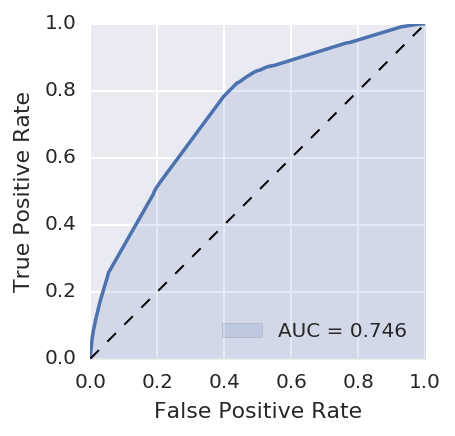
\includegraphics[width=\textwidth]{figures/roc_contacts.png}
	\caption{ROC Curve}
\label{fig:roc_contacts}
\end{subfigure}
\begin{subfigure}[t]{.49\columnwidth}
	\centering
	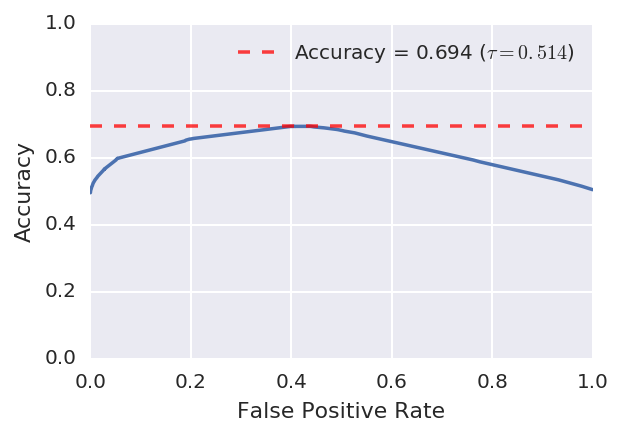
\includegraphics[width=\textwidth]{figures/accuracy_contacts.png}
	\caption{FPR-Accuracy Curve}
\label{fig:accuracy_contacts}
\end{subfigure}
\caption{The \emph{ROC Curve} and the \emph{FPR-Accuracy Curve} for the \emph{Bayesian Method} used as a comparison for the methods presented in this paper.}
\label{fig:roc_accuracy_contacts}
\end{figure}

\begin{figure}
\centering
\includegraphicsmaybe{figures/hist_contacts.png}
\caption{Distribution of $p_v$ for the \emph{Bayesian Method}, which defines the probability for a user to be part of each category.}
\label{fig:hist_contacts}
\end{figure}
